\graphicspath{{./assets/}}
\setcounter{mtc}{5}
\chapter{ 6th Sprint: Deployment of the CI/CD platform }
\fancyhead[R]{\ungaramond\small\textbf{Chapter VIII.  6th Sprint:  Deployment of the CI/CD platform }}

\minitoc
\newpage
\section*{Introduction}
Deploying a CI/CD platform is essential for modern software development as it enables developers to automate and streamline the software development lifecycle from code to production. 

In this chapter, we will discuss the process of deploying a comprehensive CI/CD platform that contains Jenkins as a CI/CD orchestrator, a SonarQube cluster for code quality and ArgoCD for continuous deployment. 

Firstly, we will go over the sprint backlog for this chapter. 

Then, we will provide an overview of the different tools and technologies that will be used in this chapter, including Jenkins, SonarQube, ArgoCD and other tools. 

Lastly, we will cover the step-by-step process of deploying the CI/CD platform. 

\section{Sprint backlog :}

\begin{longtable}[H]{|m{1.5cm}|m{3cm}|m{1.5cm}|m{9cm}|}
\hline
{\textbf{Epic ID}} & {\textbf{Epic}} & {\textbf{Story ID}} & {\textbf{Story}}\\
\hline
1  & Self-hosting the ci/cd platform tools.  &  1.1	 & Setting up the CI/CD orchestrator.\\
\cline{3-4}
& & 1.2 & Setting up the container image builder. \\
\cline{3-4}
& & 1.3	& Setting up the code quality gate. \\
\cline{3-4}
& & 1.3	& Setting up the continuous delivery controller. \\
\cline{3-4}
\hline
\end{longtable}

\section{UML design: deployment diagram for the CI/CD platform} 

The following figure illustrates the deployment diagram for the CI/CD platform we put in place to: 
\begin{enumerate}[label = (\arabic*)]
\item automate builds, tests, and deployment processes. 
\item ensure code quality. 
\end{enumerate}

\begin{figure}[H]\centering
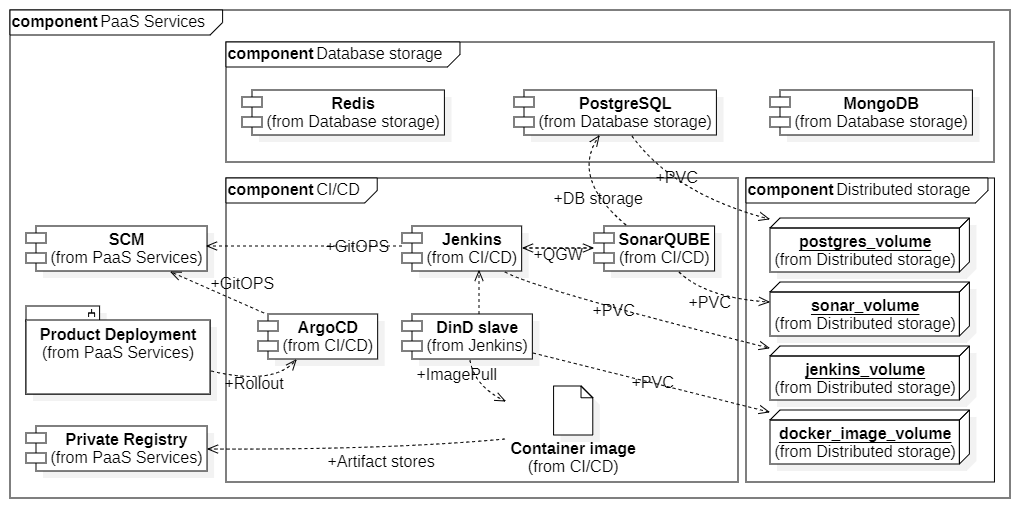
\includegraphics[width=1.0\textwidth,angle=00]{assets/f34.png}
\caption{Figure 34 }
\label{fig:f34}
\end{figure}

\section{Components of the CI/CD platform }

\subsection{The database storage backend }

When deploying databases like PostgreSQL, Redis, and MongoDB on Kubernetes, it is important to consider high availability and scalability as critical factors. 

\subsubsection{Activity diagram for deploying the database storage backend }
\begin{figure}[H]\centering
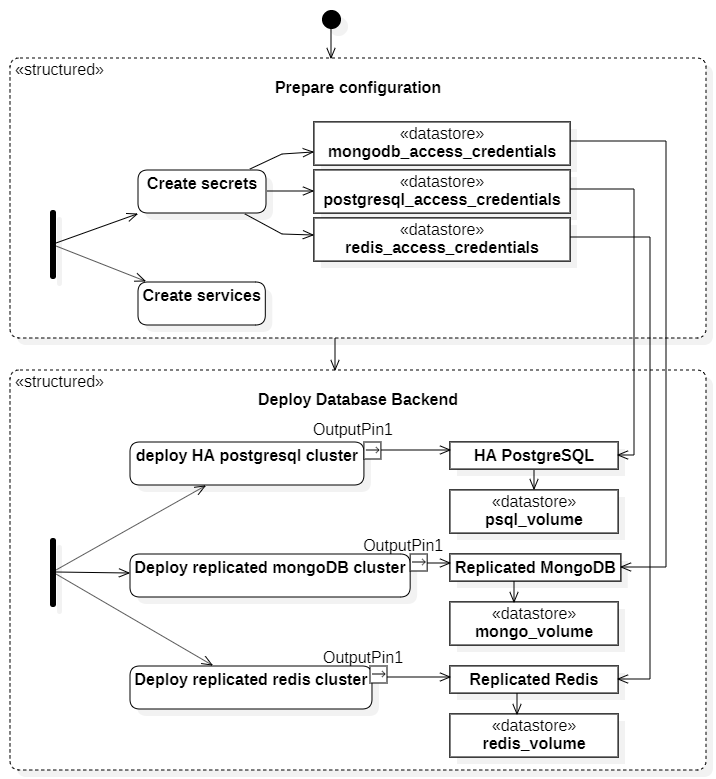
\includegraphics[width=1.0\textwidth,angle=00]{assets/f35.png}
\caption{Figure 35 }
\label{fig:f35}
\end{figure}

\subsubsection{Replicated MongoDB }

MongoDB is a popular NoSQL database that supports horizontal scaling through sharding and replication. To deploy a replicated mongodb cluster on Kubernetes, we used the following : 
\begin{itemize}[label={--}]
\item A secret that contains access credentials as well as a replica set key. 
\item Various configmaps that contain scripts for initializing the database server as well as its replicas. 
\item A statefulset for the arbiter which is a special type of node that does not store any data but participates in the election of a new primary node if the current primary node fails. 
\item A statefulset for mongodb which is configured to use environment variables as well as attachments from the created configmaps and secrets. 
\item The persistent volumes for storing data are provisioned using PersistentVolumeClaimTemplates in the statefulset. This ensures that data is preserved even if a MongoDB pod is terminated or rescheduled. 
\item A ClusterIP service for the mongodb arbiter (internal access only). 
\item NodePort services for each mongodb instance (both internal and external access to each node). 
\item A headless service (no IP) for the whole replicaSet (internal access). 
\item A LoadBalancer service for the mongodb primary instance (external access). 
\end{itemize}

Using a Kubernetes StatefulSet, we deployed multiple MongoDB instances in a replicated configuration and configured MongoDB replication for data synchronization. The following figure illustrates the workloads put in place: 


\begin{figure}[H]\centering
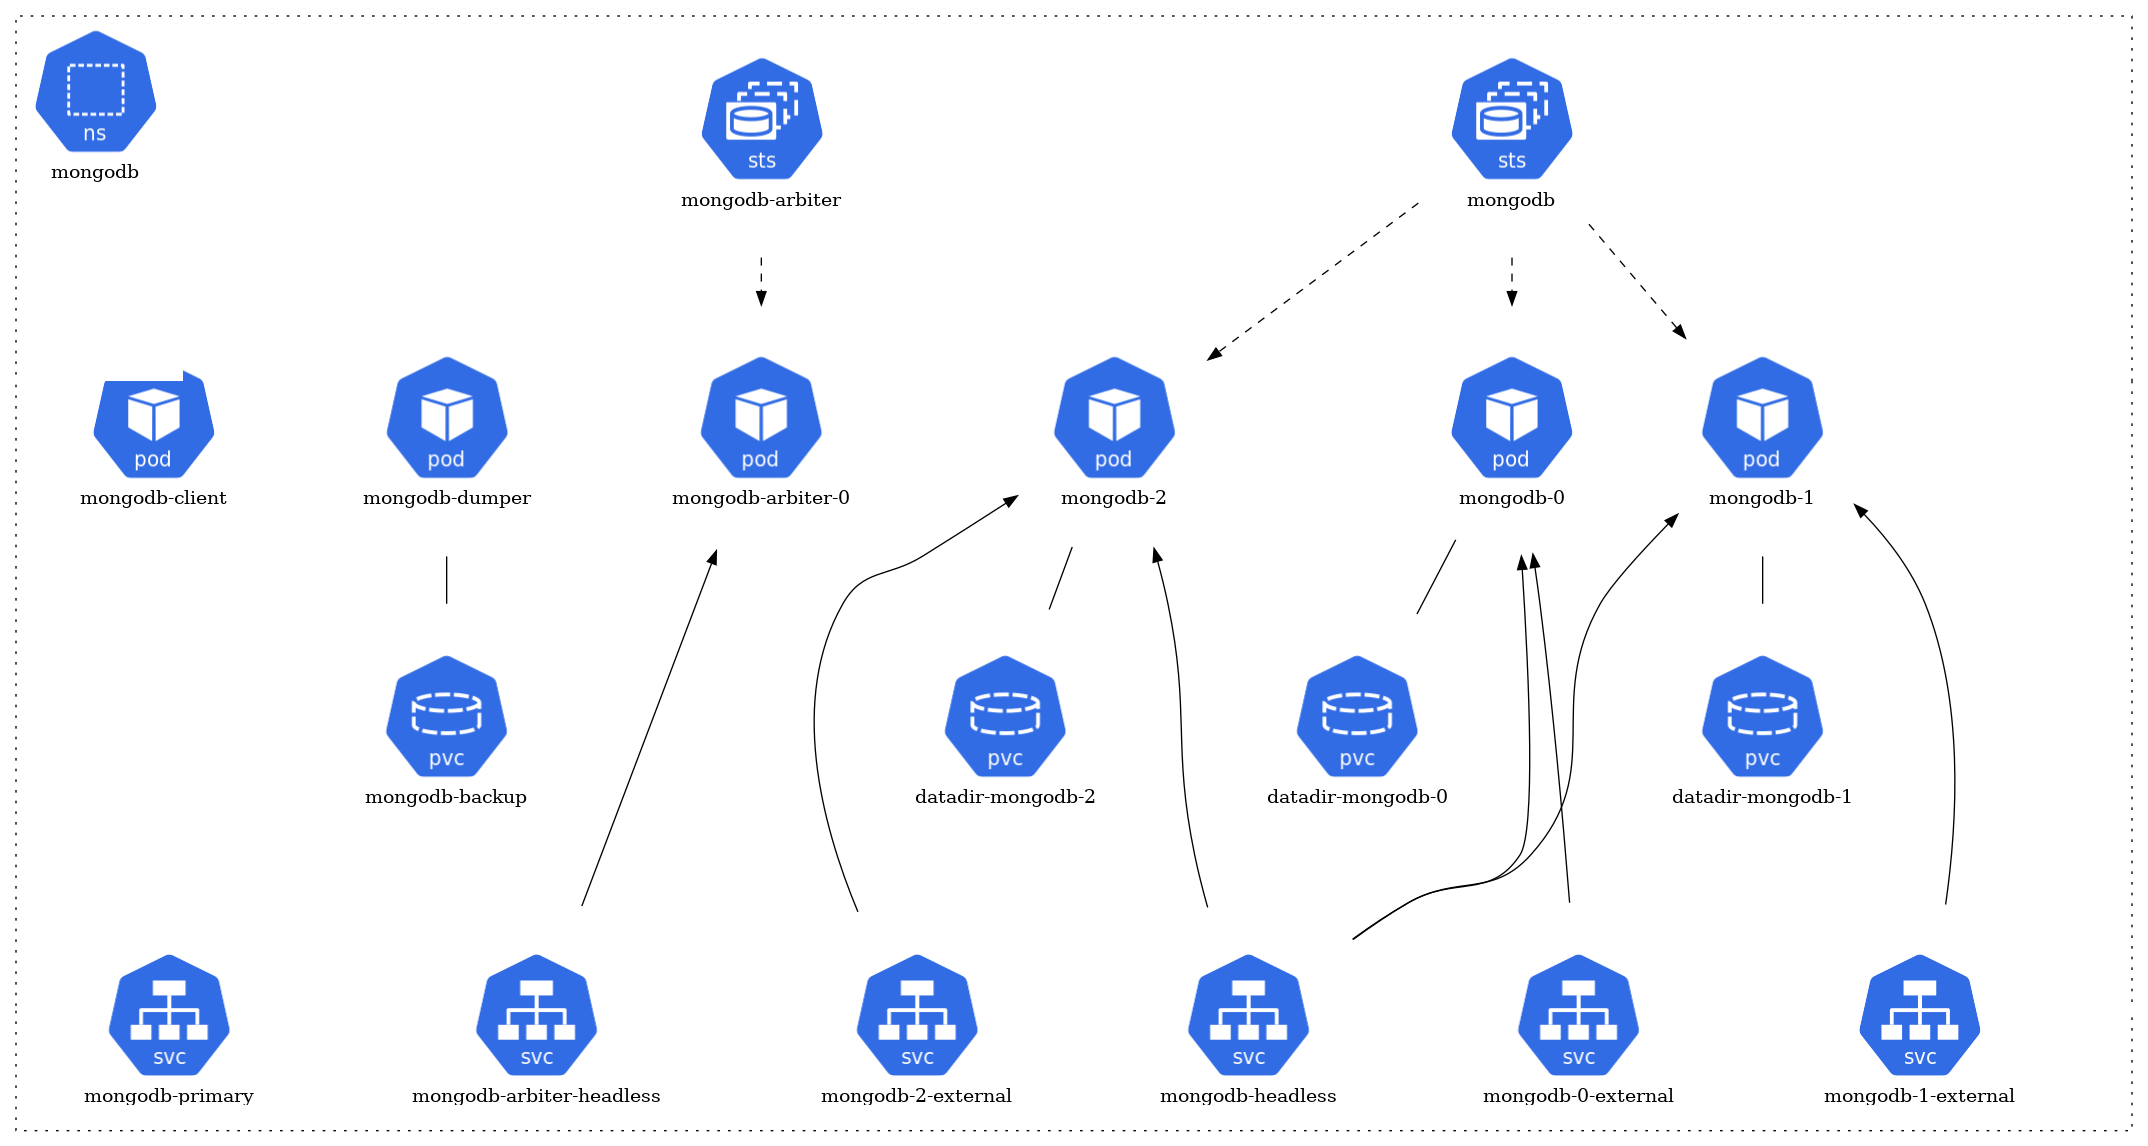
\includegraphics[width=1.0\textwidth,angle=00]{assets/f36.png}
\caption{Figure 36 }
\label{fig:f36}
\end{figure}

With this setup, you can have a highly available and scalable MongoDB database infrastructure for your containerized applications. 

 
\subsubsection{HA PostgreSQL }

Highly Available (HA) PostgreSQL on Kubernetes involves deploying multiple PostgreSQL instances that are managed by Kubernetes and are configured in a primary-standby replication configuration.  

To deploy PostgreSQL in a highly available configuration on Kubernetes, we used the following : 
\begin{itemize}[label={--}]
\item A secret that contains access credentials as well as a password for the replication manager. 
\item a configmap that contains scripts for initializing the database server as well as its replicas. 
\item A statefulset that guarantees the ordering and uniqueness of pod identities for postgreql. 
\item A Pgpool-II statefulset that is used in conjunction with PostgreSQL and acts as a middleman between the client applications and the PostgreSQL database. It can also monitor the health of the PostgreSQL instances and promote a standby node to a primary node in case of a failure. 
\item The persistent volumes for storing data are provisioned using PersistentVolumeClaimTemplates in the statefulset. This ensures that data is preserved even if a PostgreSQL pod is terminated or rescheduled. 
\item A NodePort service for the pgpool service (internal access only). 
\item  A headless service (no IP) for the whole replicaSet (internal access). 
\end{itemize}

With this setup, we deployed a highly available and scalable PostgreSQL database infrastructure for containerized applications. The following figure illustrates the workloads put in place: 

\begin{figure}[H]\centering
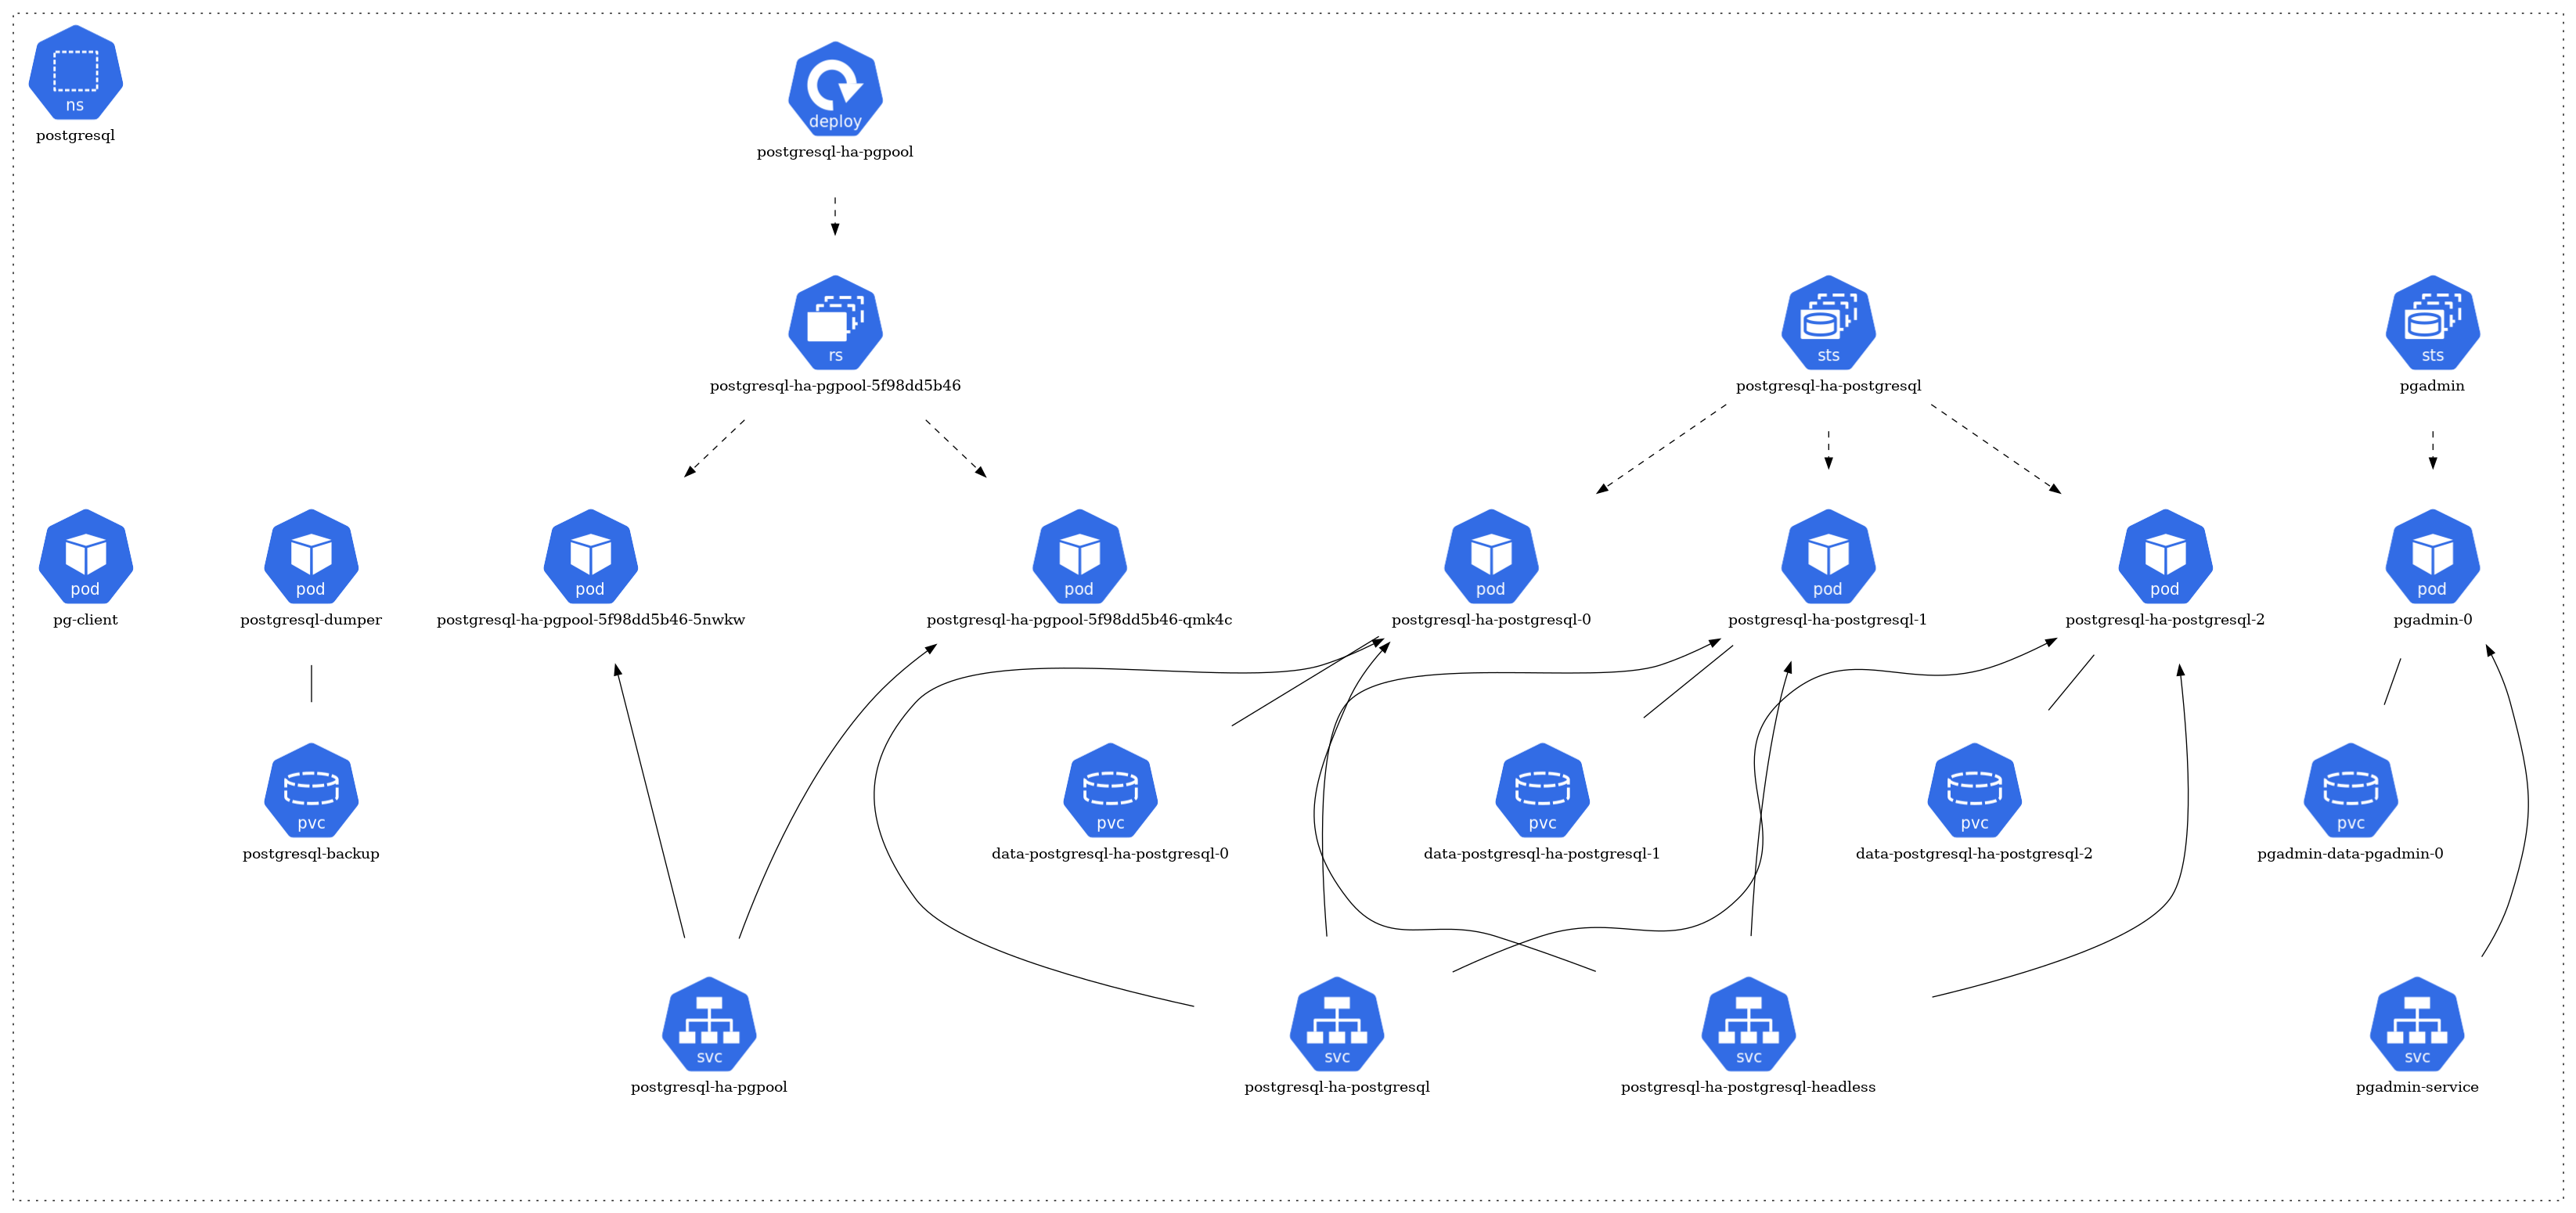
\includegraphics[width=1.0\textwidth,angle=00]{assets/f37.png}
\caption{Figure 37 }
\label{fig:f37}
\end{figure}

This configuration ensures that one PostgreSQL instance always serves as the primary node that accepts all writes and updates, while the other instances act as standby nodes that replicate data from the primary node. 

\subsubsection{Replicated Redis }

Redis is an in-memory data structure store used as a database, cache, and message broker. 
\begin{itemize}[label={--}]
\item In a similar fashion to HA postgresql, deploying a replicated Redis cluster on Kubernetes involves: 
\item using a Kubernetes StatefulSet to deploy multiple Redis instances in a replicated configuration, 
\item configuring Redis replication for data synchronization, 
\item using a Kubernetes Service to provide a stable endpoint for accessing the Redis cluster, 
\item and using a Kubernetes PVC to ensure data persistence. 
\end{itemize}
With this setup, you can have a highly available and scalable Redis database infrastructure for your containerized applications. 

The resulting setup is illustrated by the following figure: 

\begin{figure}[H]\centering
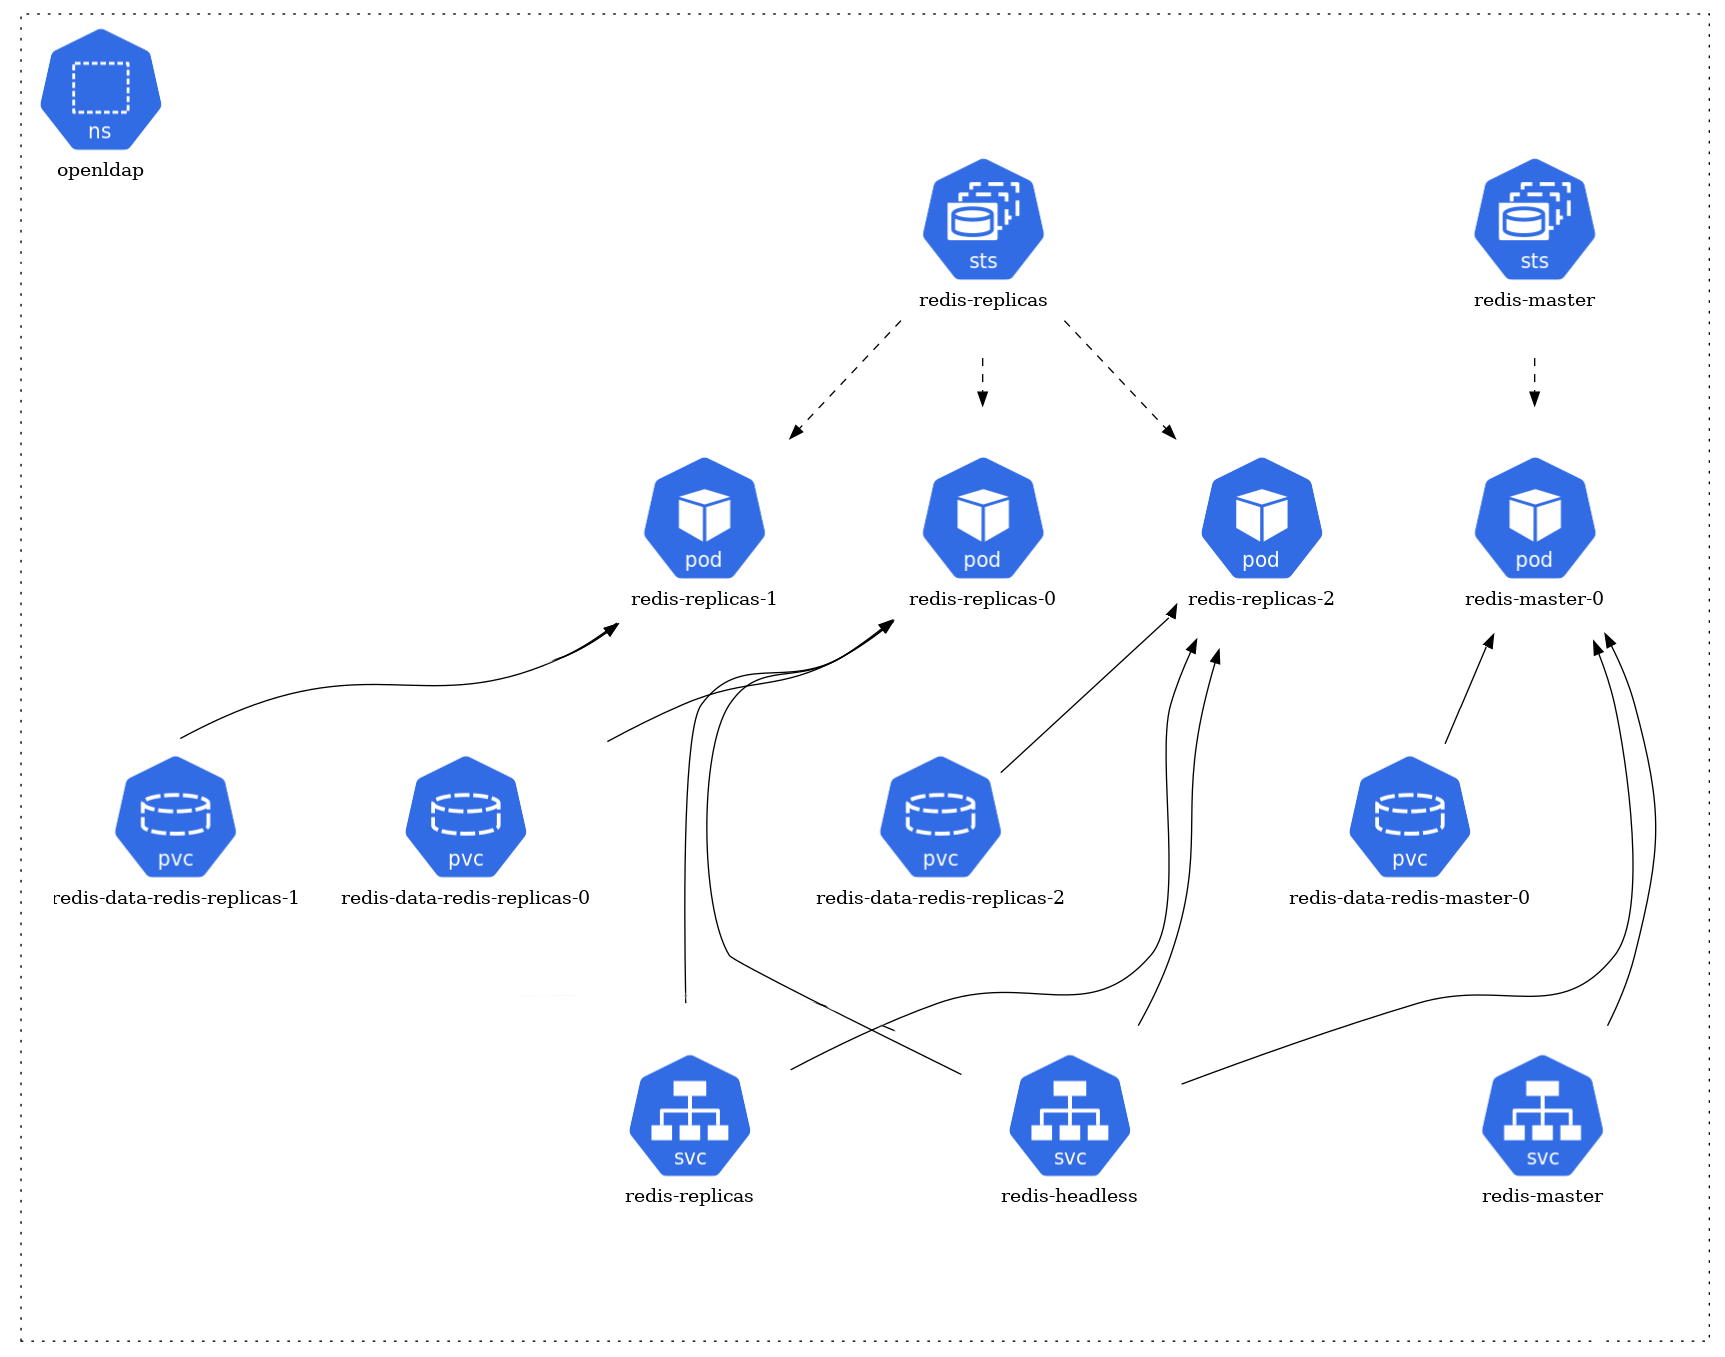
\includegraphics[width=1.0\textwidth,angle=00]{assets/f38.png}
\caption{Figure 38 }
\label{fig:f38}
\end{figure}


\section*{Conclusion}
